% Created 2019-03-06 Wed 10:48
% Intended LaTeX compiler: pdflatex
\documentclass[11pt]{article}
\usepackage[utf8]{inputenc}
\usepackage[T1]{fontenc}
\usepackage{graphicx}
\usepackage{grffile}
\usepackage{longtable}
\usepackage{wrapfig}
\usepackage{rotating}
\usepackage[normalem]{ulem}
\usepackage{amsmath}
\usepackage{textcomp}
\usepackage{amssymb}
\usepackage{capt-of}
\usepackage{hyperref}
\author{Eskild Trøen, Amalie Hennie, Sindre Sivertsen, Simen Holmestad}
\date{\today}
\title{Innlevering 1: Konseptuell databasemodell}
\hypersetup{
 pdfauthor={Eskild Trøen, Amalie Hennie, Sindre Sivertsen, Simen Holmestad},
 pdftitle={Innlevering 1: Konseptuell databasemodell},
 pdfkeywords={},
 pdfsubject={},
 pdfcreator={Emacs 26.1 (Org mode 9.1.9)},
 pdflang={English}}
\begin{document}

\maketitle

\section*{A) ER-diagram}
\label{sec:orgf8c3814}
\href{file:///Users/simen/Dropbox/skole/v\%C3\%A5r2019/databaser/\%C3\%B8vinger/Brominator/ER-diagram\_treningsdagbok\_picture.png}{\begin{figure}[htbp]
\centering
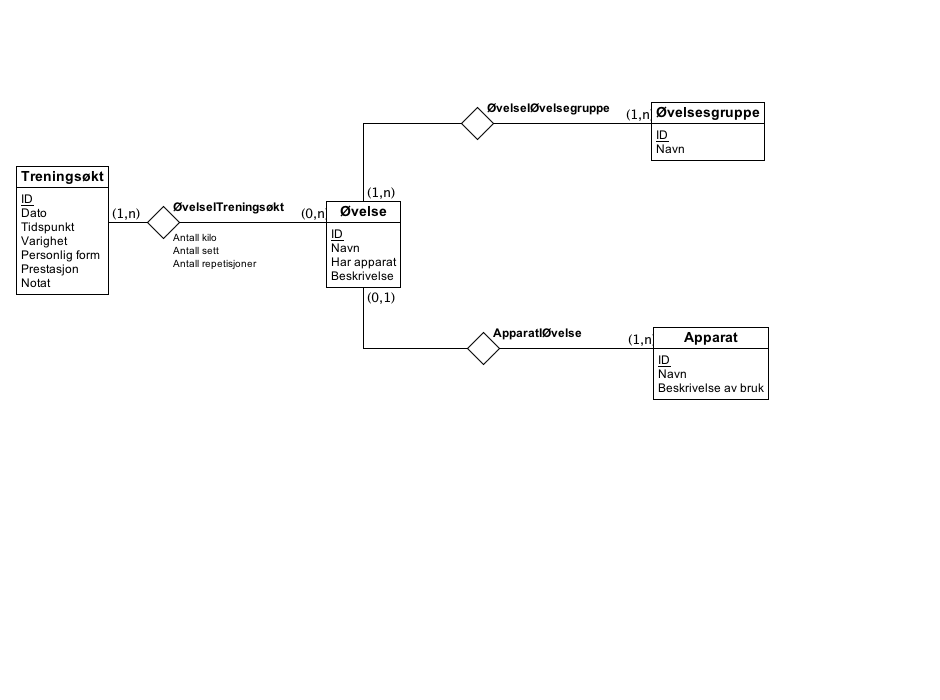
\includegraphics[width=.9\linewidth]{../ER-diagram_treningsdagbok_picture.png}
\bicaption{ER-diagram}
\end{figure}}\\

\subsection*{Antagelser:}
\label{sec:orge150a5a}
\begin{itemize}
\item Databasen er treningsdagboken til én bruker\\
\item En øvelse er en generell øvelse og ikke spesifikk for en treningsøkt\\
\item En øvelse er en apparatøvelse hvis HarApparat er true.\\
\item Hvis en øvelse ikke er en apparatøvelse kan attributtene i ØvelseITreningsøkt settes til null\\
\end{itemize}
\section*{B) Relasjonsdatabasemodell}
\label{sec:org2d67107}
\begin{itemize}
\item Treningsøkt( \uline{TreningsøktID}, Dato, Tidspunkt, Varighet, PersonligForm, Prestasjon, Notat )\\
\item Øvelse( \uline{ØvelseID}, Navn, Beskrivelse, HarApparat, ApparatID )\\
\item ØvelseITreningsøkt( \uline{TreningsøktID}, \uline{ØvelseID} Kilo, AntallSett, AntallReps )\\
\item Apparat( \uline{ApparatID}, Navn, HvordanBruke )\\
\item Øvelsesgruppe( \uline{ØvelsesgruppeID}, Navn )\\
\item ØvelseIØvelsesgruppe( \uline{ØvelsesgruppeID}, \uline{ØvelseID} )\\
\end{itemize}

Vi valgte å modellere Kilo, AntallSett og AntallReps på relasjonen mellom Øvelse og Treningsøkt fordi øvelsene da kan være generelle øvelser og at man slipper å opprette nye øvelser for hver treningsøkt. Når vi kobler økt mot øvelse vil vi da også få med hvor bra det gikk på de forskjellige øvelsene akkurat denne treningsøkten.\\

\section*{C) Hvordan oppfylle krav}
\label{sec:org6912393}
Oppgave: For hvert nummerert punkt i kravspesifikasjonen skal det kort forklares hvordan modellen deres oppfyller kravet til en slik funksjonalitet.\\
\subsection*{1. Registrering}
\label{sec:org48ae982}
Vi har tabeller i SQL som kan registrere apparatoer, øvelser og treningsøkter med tilhørende data.\\
\subsection*{2. Få opp informasjon om n siste treningsøkter}
\label{sec:orgd04294e}
Her kan vi selecte treningsøkter på ID så vi får ut de n siste og kan vise informasjon om dette.\\
\subsection*{3. Resultatlogg av øvelser i tidsintervall}
\label{sec:org3eb238c}
Ved å joine Øvelse og Treningsøkt på gitt dato (og evt. tidspunnkt) på dato (og tidspunkt) kan vi får ut øvelsene gjennomført i det gitte tidsrommet. Man kan se ulik prestasjon i antall kilo, sett og reps i relasjonen mellom Treningsøkt og Øvelse.\\
\subsection*{4. Finne øvelser i samme øvelsesgruppe}
\label{sec:org4e14568}
Vi har testdata lagt inn i databasen som kan brukes til å teste med. Siden alle øvelser må ha lagt inn hvilke(n) øvelsesgruppe den er i, kan man opprette en øvelsesgruppe og sjekke om øvelsen har den gitte øvelsesgruppa.\\
\subsection*{5. Valgfritt use case}
\label{sec:org718b0e5}
Få informasjon om totalt antall kilo løftet, repetisjoner og sett utført av brukeren. Gjennom ØvelseITReningsøkt-tabellen har vi tilgang til alle øvelser utført av brukeren og attributtene Kilo, AntallSett og AntallReps. En summering over radene i de respektive kolonnene vil gi ønske resultat.\\
\section*{D) SQL-script}
\label{sec:org3b34255}
\begin{verbatim}
DROP TABLES IF EXISTS Treningsøkt, Øvelse, Apparat, ØvelsesGruppe,
ØvelseITreningsøkt, ØvelseIØvelsesgruppe;
CREATE TABLE Treningsøkt (
    TreningsøktID INTEGER NOT NULL AUTO_INCREMENT,
    Dato DATETIME NOT NULL,
    Varighet TIME NOT NULL,
    PersonligForm INTEGER NOT NULL,
    Prestasjon INTEGER NOT NULL,
    Notat TEXT NOT NULL,
    CONSTRAINT Treningsøkt_PK PRIMARY KEY (TreningsøktID)
);
CREATE TABLE Apparat (
    ApparatID INTEGER NOT NULL AUTO_INCREMENT,
    Navn VARCHAR(30) NOT NULL,
    HvordanBruke TEXT NOT NULL,
    CONSTRAINT Apparat_PK PRIMARY KEY (ApparatID)
);
CREATE TABLE Øvelse (
    ØvelseID INTEGER NOT NULL AUTO_INCREMENT,
    Navn VARCHAR(30) NOT NULL,
    Beskrivelse TEXT NOT NULL,
    HarApparat BOOLEAN NOT NULL,
    ApparatID INTEGER NOT NULL,
    CONSTRAINT Øvelse_PK PRIMARY KEY (ØvelseID),
    CONSTRAINT Øvelse_FK FOREIGN KEY (ApparatID)
	REFERENCES Apparat (ApparatID)
	ON UPDATE CASCADE ON DELETE CASCADE
);
CREATE TABLE ØvelsesGruppe (
    ØvelsesgruppeID INTEGER NOT NULL AUTO_INCREMENT,
    Navn VARCHAR(30) NOT NULL,
    CONSTRAINT ØvelsesGruppe_PK PRIMARY KEY (ØvelsesgruppeID)
);
CREATE TABLE ØvelseITReningsøkt (
    TreningsID INTEGER NOT NULL AUTO_INCREMENT,
    ØvelseID INTEGER NOT NULL,
    Kilo FLOAT(24),
    AntallSett INTEGER,
    AntallReps INTEGER,
    CONSTRAINT ØvelseITReningsøkt_PK PRIMARY KEY (TreningsID , ØvelseID),
    CONSTRAINT ØvelseITReningsøkt_FK1 FOREIGN KEY (TreningsID)
	REFERENCES Treningsøkt (TreningsøktID)
	ON UPDATE CASCADE ON DELETE CASCADE,
    CONSTRAINT ØvelseITReningsøkt_FK2 FOREIGN KEY (ØvelseID)
	REFERENCES Øvelse (ØvelseID)
	ON UPDATE CASCADE ON DELETE CASCADE
);
CREATE TABLE ØvelseIØvelsesgruppe (
    ØvelseID INTEGER NOT NULL AUTO_INCREMENT,
    ØvelsesgruppeID INTEGER NOT NULL,
    CONSTRAINT ØvelseIØvelsesgruppe_PK PRIMARY KEY (ØvelseID , ØvelsesgruppeID),
    CONSTRAINT ØvelseIØvelsesgruppe_FK1 FOREIGN KEY (ØvelseID)
	REFERENCES Øvelse (ØvelseID)
	ON UPDATE CASCADE ON DELETE CASCADE,
    CONSTRAINT ØvelseIØvelsesgruppe_FK2 FOREIGN KEY (ØvelsesgruppeID)
	REFERENCES ØvelsesGruppe (ØvelsesgruppeID)
	ON UPDATE CASCADE ON DELETE CASCADE
);
\end{verbatim}
\end{document}
